\documentclass[journal]{./IEEE/IEEEtran}
\usepackage{cite,graphicx,textcomp,float}


\newcommand{\SPTITLE}{UPLB Alumni System: An Online Yearbook and Social Network for UPLB Alumni}
\newcommand{\ADVISEE}{Leo Angelo C. Diabordo}
\newcommand{\ADVISER}{Katrina Joy Magno}

\newcommand{\BSCS}{Bachelor of Science in Computer Science}
\newcommand{\ICS}{Institute of Computer Science}
\newcommand{\UPLB}{University of the Philippines Los Ba\~{n}os}
\newcommand{\REMARK}{\thanks{Presented to the Faculty of the \ICS, \UPLB\
                             in partial fulfillment of the requirements
                             for the Degree of \BSCS}}
        
\markboth{CMSC 190 Special Problem, \ICS}{}
\title{\SPTITLE}
\author{\ADVISEE~and~\ADVISER%
\REMARK
}
\pubid{\copyright~2014~ICS \UPLB}

\begin{document}

% TITLE
\maketitle


% INTRODUCTION
\section{Introduction}

\subsection{Background of the Study}
Books have been very useful in storing and disseminating information since papermaking was invented in AD 105 \cite{electronic_eb_papermaking}. However, their accessibility is greatly limited due to their physical nature. With today$'$s modern technology, books have been digitized in great quantities through mass digitization projects such as the Google Books Library Project \cite{electronic_glibproj} and the Open Content Alliance \cite{electronic_oca} in an effort to “remove the barriers between people and information” \cite{electronic_glibproj_perspective} and to “build a permanent archive of multilingual digitized text and multimedia content” \cite{electronic_oca_about}

Electronic books (eBooks) are one example of the result of digitization, and although newer printed books are simultaneously produced with their digital counterpart, older books will either undergo document scanning and Optical Character Recognition or a total re-encoding of its contents.
Digitization of books are not only limited to journals, novels, and other text-heavy materials. Yearbooks, whose contents mainly consist of relevant information on the graduating class and a portrait of each fresh graduates, have also been digitized in Universities \cite{article_51_yearbooks}. \par

Developing the UPLB Alumni System offers the convenience of accessing information on UPLB graduates in a single environment. The UPLB Alumni System will not only be a website hosting digitized copy of UPLB yearbooks but will also offer social networking features that will focus on helping its users establish connections with other UPLB graduates for the expansion of their professional network. \par

There are already a number of existing career-oriented social networks such as LinkedIn and even more websites for online job postings. Some companies also accept job applications through email. But with the millions of people who have access to these websites and are capable of sending their applications in seconds, recruits also have lesser time to evaluate all of the resumes they receive and so some end up not getting evaluated at all\cite{6615172220111003}. \par

\subsection{Statement of the Problem}
Yearbooks are usually produced in numbers equal to the number of graduates for the academic year, this presents the problem of having a limited number of copies of the book and limited access to them. \par

In most cases, the production of UPLB yearbooks is initiated by the college student councils. Thus, the yearbooks are decentralized. Packages are usually offered to the graduating students. This includes a pictorial session and a copy of the yearbook, costing around 2,000 pesos. Since the publication of yearbooks in UPLB is not officially handled by the University, purchasing of the yearbook is not part of the requirements for graduation. It is entirely up to the student if they will avail of the package offered or not. Choosing the latter would mean that they will not have a photo in the yearbook. Because purchasing of yearbooks is optional, some students choose to either only avail of a copy of the yearbook or to not avail at all. Thus, some graduates are not included in the yearbook. \par

\subsection{Significance of the Study}
The proposed study will focus on bringing information about the 51,882 alumni UPLB have produced (as of March 2014) \cite{electronic_oar} in a more accessible medium, the Internet, and in the process would make stronger relations among the alumni and to help increase their professional network. By bringing features that will make professional relations easier such as recommending a person to a company or advertising vacant position in the user's current company, UPLB Alumni System will not only serve as a database for alumni information but also offer career-oriented networking. UPLB Alumni System will also address the problem of having too much competing CVs when applying for jobs by using recommendations from other users as leverage. The system will also provide updated information from active users to the GTracer system. The GTracer system will be a graduate tracer system that aims to help the Office of Student Affairs keep track of the progress of students after they have graduated. \par

\subsection{Objectives}
The main objective of the study is to develop a web application that will act as a social network accessible only to UPLB graduates and an online yearbook that can be freely accessed by anyone through the Internet, and to develop the system such that it can be released as an open source software to other universities who will have to maintain their own database of users. The following are the specific objectives:
	\begin{enumerate}
	\item To use the Application Programming Interface (API) of the Office of Student Affairs Management (OSAM) System to create an initial profile for each alumni
	\item To allow the users to create connections with other users \pubidadjcol
	\item To implement a smart-suggest feature to notify the user of possible connections of interest based on the user's details, such as course, majors, organizations, etc.
	\item To create UPLB Alumni System's own API so that other systems will have access to some of the functionalities and data from the it. 
	\end{enumerate}

\subsection{Scope and Limitation}
The online yearbook feature of the UPLB Alumni System will be available to anyone who has Internet access, however, only UPLB graduates will have access to the social network feature of the system. The UPLB Alumni System will not have a sign up option, since the creation of account will be handled by the administrators of the system. The social networking feature will focus on obtaining work-related information (e.g. current workplace, employment history) of the said individuals. \par

% REVIEW OF RELATED LITERATURE
\section{Review of Related Literature}
Social networks are made up of group of people that interact with each other to achieve certain goals\cite{wpangako}. These goals have a wide array of categories to fall onto, such as language learning, sharing of experiences, work collaborations, etc.
Together with the rise of the Internet, web-based social networks have sprung out. And by utilizing the services that the Internet offered as its medium, web-based social networks have had a further reach in connecting people \textendash \.even transcending geographic borders\cite{comscore}. More and more social networking websites have also surfaced each having a different focus such as on microblogging, photo and video sharing,  green living and social activism, and many more. \par
Of the many web-based social networks available to date, Facebook still tops the list with the most monthly active users at 1.35 billion monthly active users as of September 30, 2014\cite{fb}, followed by Google+ at 540 million\cite{ny}, Twitter with 284 million monthly active users\cite{twitter}, Instagram with 200 million\cite{insta} and LinkedIn with 187 million\cite{seekingalpha}. Among the top 5 social networking websites who cater towards the general idea of networking, microblogging, and media sharing, LinkedIn stands out by focusing on business and professional networking.\par
According to a study conducted across the United States by Achievers (formerly I Love Rewards®) on the graduating class of 2012, “35\% plan to utilize LinkedIn as their top social media platform to look for a job”\cite{achievers12}. This figure increased by 29 percent on their latest comprehensive survey on the graduating class of 2013\cite{achievers13}. Possibly one reason for the gaining popularity of LinkedIn and one of the advantage in using similar professional networking services is that, with the public availability of the information provided by the users for their resume, claims written in the users’ resume require greater honesty especially on verifiable information and less on unverifiable information. Compared to people using a traditional resume, it is the opposite of the previous scenario, those who made and used traditional resumes lied more on verifiable information and less on unverifiable information, presumably because there is lesser risk of being caught and information deemed important by both the applicant and the employer such as work history are verifiable.\cite{7316265520120301}\par
With the rate of unemployment in the country at 7.5 percent, and underemployment rate at 19.5 percent, it is not a surprise if some people would alter information presented in their resume to be more appealing towards the employer.\cite{ble}\par
Another popular practice that gained momentum during the recent years is Job Hopping. Job hopping is the term used when an employee does not stay in the company for longer than a year or two. A survey conducted by CareerBuilder among 2,138 hiring managers and Human Resources (HR) professionals, and 3022 workers showed that more than 55 percent of employers hired a job hopper and 32 percent said that they are expecting workers to job hop\cite{jobhop}. Another study by The Marketer’s Forum found that 42 percent left their jobs after 18 months since starting, and 20 percent quit after just six months. The respondents’ reason for quitting their job quickly revolved around not being able to “progress up the career ladder fast enough”. Many also used their first job to try out the industry and 15 percent of them realized that they had picked the wrong career\cite{gfog}. \\ \par

{\setlength{\parindent}{0pt}
\setlength{\parskip}{\baselineskip}
\textit{Some Universities that have Online Copies of their Digitized Yearbooks}}

\begin{enumerate}
	\item University of Maryland \\
	\textendash \, The University Archives of the University of Maryland contains digitized copies of yearbooks dating from 1897 and are available for online viewing and for download in Portable Document Format (PDF). \cite{UM}\\

	\item University of Pennsylvania: Penn \\
	\textendash \, The website of the University$'$s University Archives and Records Center offers downloadable copies of their undergraduate yearbooks. Twentieth century yearbooks are available in 10 year bundles, and while earlier yearbooks of the nineteenth century are also available, copies of yearbooks for each year since 1863 are not all available. \cite{UP}\\

	\item University of Iowa \\
	\textendash \, The University of Iowa Libraries hosts digitized copies of the University$'$s Hawkeye yearbook. Yearbooks published from 1892\textendash 1992 are available for online viewing only. \cite{UI}\\

	\item University of Delaware \\
	\textendash \, The University of Delaware Libraries has a collection of yearbooks published by students of Delaware College and later the University of Delaware. Copies of the yearbooks are available for downloading by chapter. \cite{UD}\\

	\item Creighton University \\
	\textendash \, Copies of Creighton$'$s University yearbook, the Bluejay, are available through Creighton University$'$s online resources. Digitized copies of the yearbooks are hosted by the Internet Archive and is available for online viewing and also for download in multiple formats. \cite{CU}\\

	\item University of Nebraska \\
	\textendash \, The Archives of the University of Nebraska-Lincoln Libraries contains digitized copies of all of the University$'$s yearbooks from 1884 and can be viewed online, with some copies being searchable. \cite{UN}\\
	\end{enumerate}


% METHODOLOGY
\section{Methodology}
\subsection{Development Tools}
In order to implement the system, the following are necessary:
\begin{enumerate}
	\item Programming Language: PHP 5.4.12 will be used as the programming language of the system. PHP is a general-purpose scripting language that is popularly used for web development.
	\item Database: The database that will be used by system will be MySQL 5.6.12 MySQL is an open-source relational database management system and is currently the database used by the OSAM system. Using the same database as the OSAM system will ensure compatibility and an easier way of accessing information from the OSAM system.
	\item Front-end Framework: Foundation will be used in building and customizing the front-end of the system.
\end{enumerate}

\subsection{Functional Requirements}
	
The system is to be used by three (3) types of users; the Administrator, the Alumni, and the Guests. Each user will be given different privileges in using the system.
		\begin{enumerate}
			\begin{figure} 
				\centering
				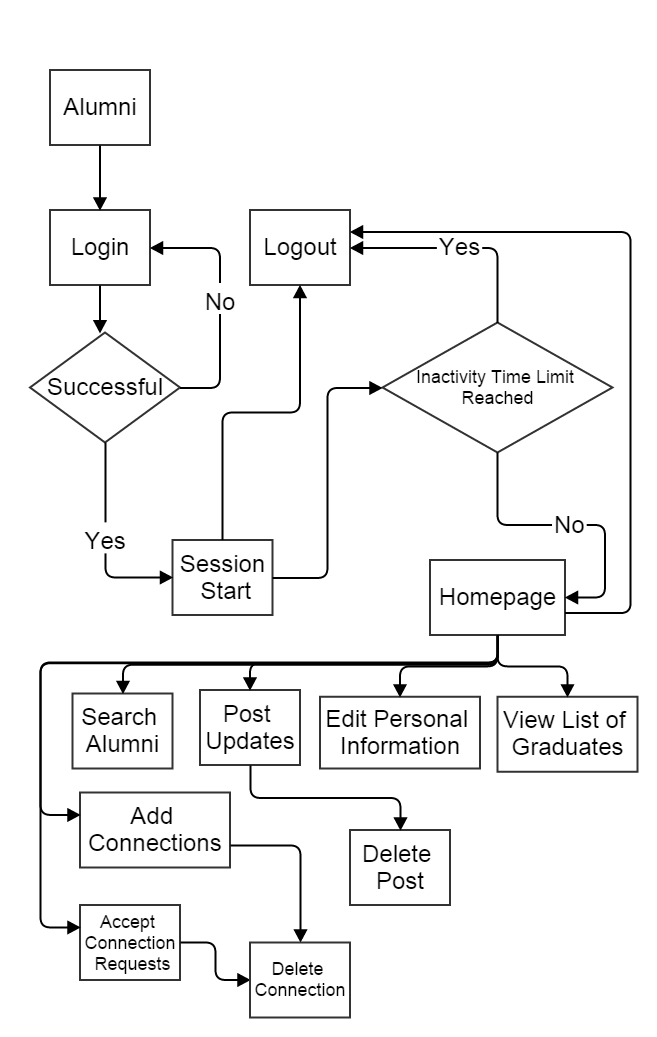
\includegraphics[width=9cm,height=13cm]{Images/AlumniFlowChart.png}
				\caption{Alumni Workflow Diagram}
			\end{figure}
			\item An Alumni will be able to use the following functionalities of the system:
				\begin{itemize}
				\item Request and/or remove connections with other alumni
				\item Approve or decline requests of connections from other alumni
				\item Update personal information
				\item Change account password
				\item Create and/or remove posts
				\item Search and view alumni by:
					\begin{itemize}
					\item Name
					\item Course
					\item Affiliated Organizations
					\item Year of Graduation
					\item Workplace
					\end{itemize}
				\item Request for the addition of a missing school/academy/university in the list of previous schools
				\item Request for the addition of a company that is not included in the list of companies
				\item View all UPLB graduates using the yearbook page
				\end{itemize}
			\begin{figure} 
				\centering
				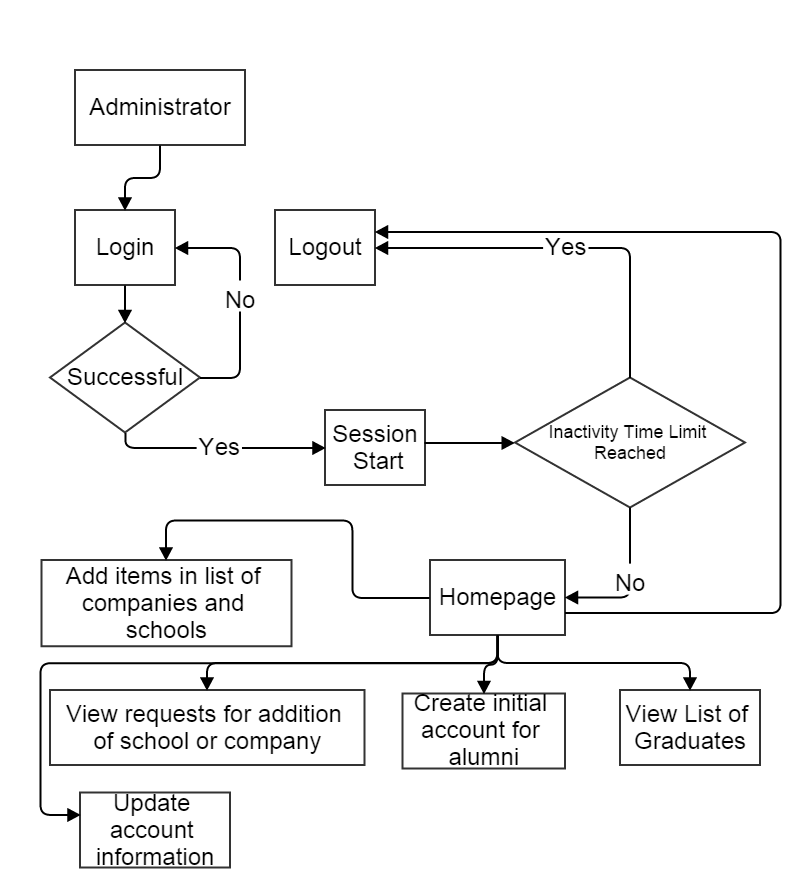
\includegraphics[width=8cm,height=9cm]{Images/AdminFlowChart.png}
				\caption{Administrator Workflow Diagram}
			\end{figure}
			\item Administrators of the system will have the following privileges:
				\begin{itemize}
				\item Add a school in the list of schools that users can add as their former school
				\item Add a company in the list of companies
\begin{figure*}
			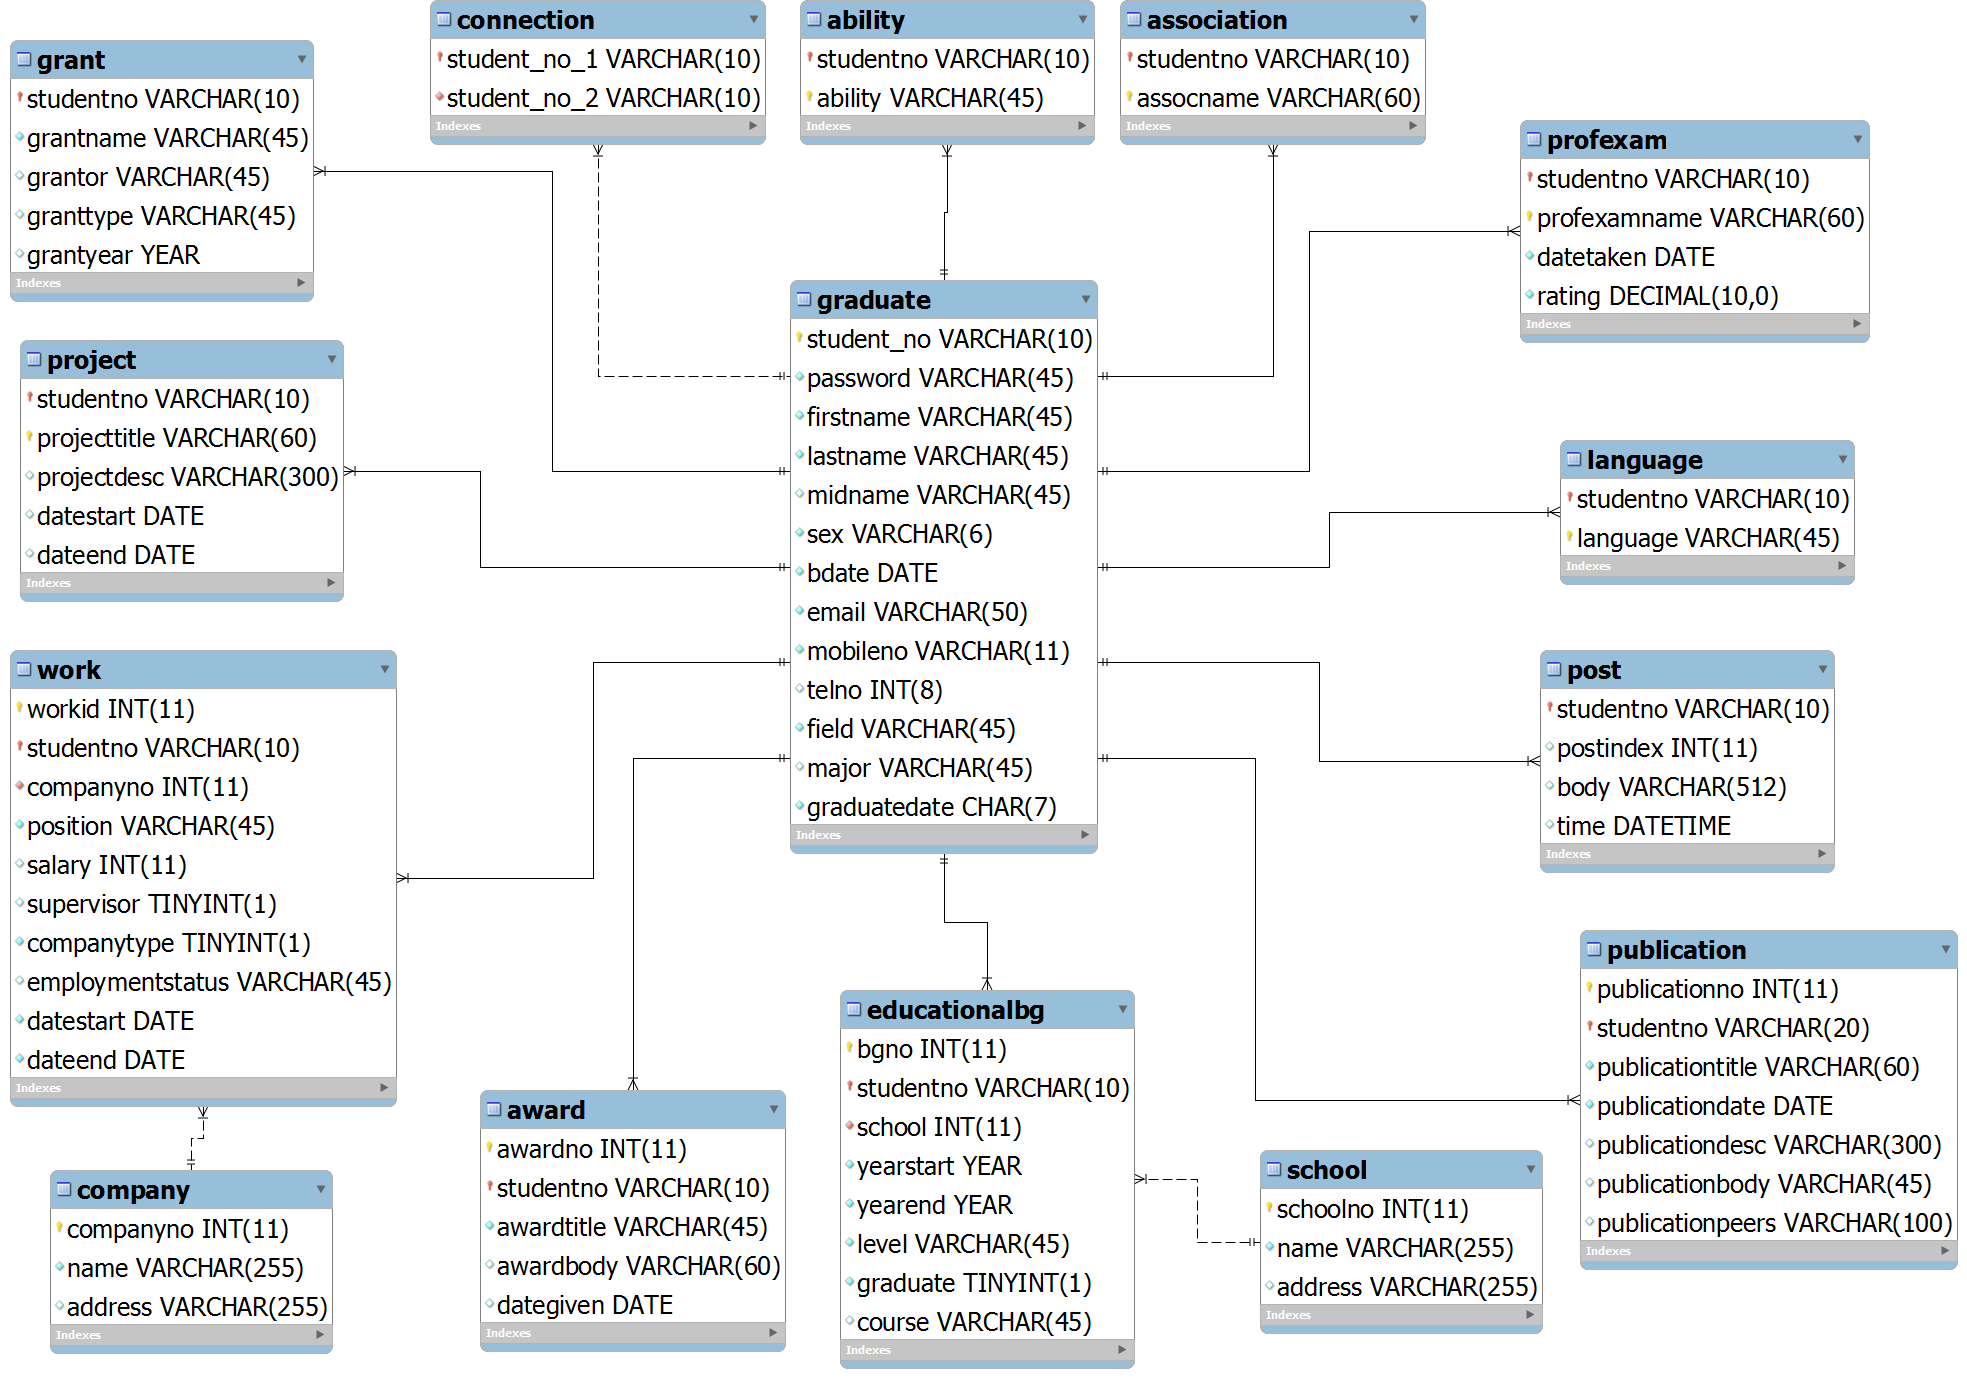
\includegraphics[width=18cm,height=12cm]{Images/UML5.png}
			\caption{Unified Modeling Language Class Diagram}
		\end{figure*}
				\item Create initial accounts of alumni
				\item View requests for addition of company or school in respective lists
				\end{itemize}
			\item Guests will only be able to access the online yearbook page of the system. They will also have access to the following features:
				\begin{itemize}
				\item View the online yearbooks
				\item Search an alumni by:
					\begin{itemize}
					\item Name
					\item Course
					\item Year of Graduation
					\end{itemize}
				\end{itemize}
		\end{enumerate}
		
\subsection{System Design}
	In creating the System Design,  generation of a Unified Modeling Language (UML) diagram was necessary to provide a visual representation of the database that the system will be using. The UML diagram also shows the connection between the entities in the database as shown in Figure 3.
		

		The Administrator creates the accounts of alumni by using the API of the OSAM system to obtain basic information such as full name, student number, year of graduation, and organizations that the alumnus/alumna is affiliated with.
		The Alumni can then log in to their initial accounts and will be asked to change their initial password. the Alumni will also be asked to update information such as current workplace, etc. After logging in, an Alumni will be able to post updates in his Homepage that other Alumni in his\slash her connections list can see. Alumni users will also be able to use the search function of the system to search for people they know, and to limit the scope of their search(e.g., within their affiliated organizations, specified year of graduation, or workplace). 
% INITIAL RESULTS
\section{Initial Results}
{\setlength{\parindent}{0pt}
\setlength{\parskip}{\baselineskip}
\textit{Mockup User Interface}}

\begin{figure}[H]
\begin{center}
		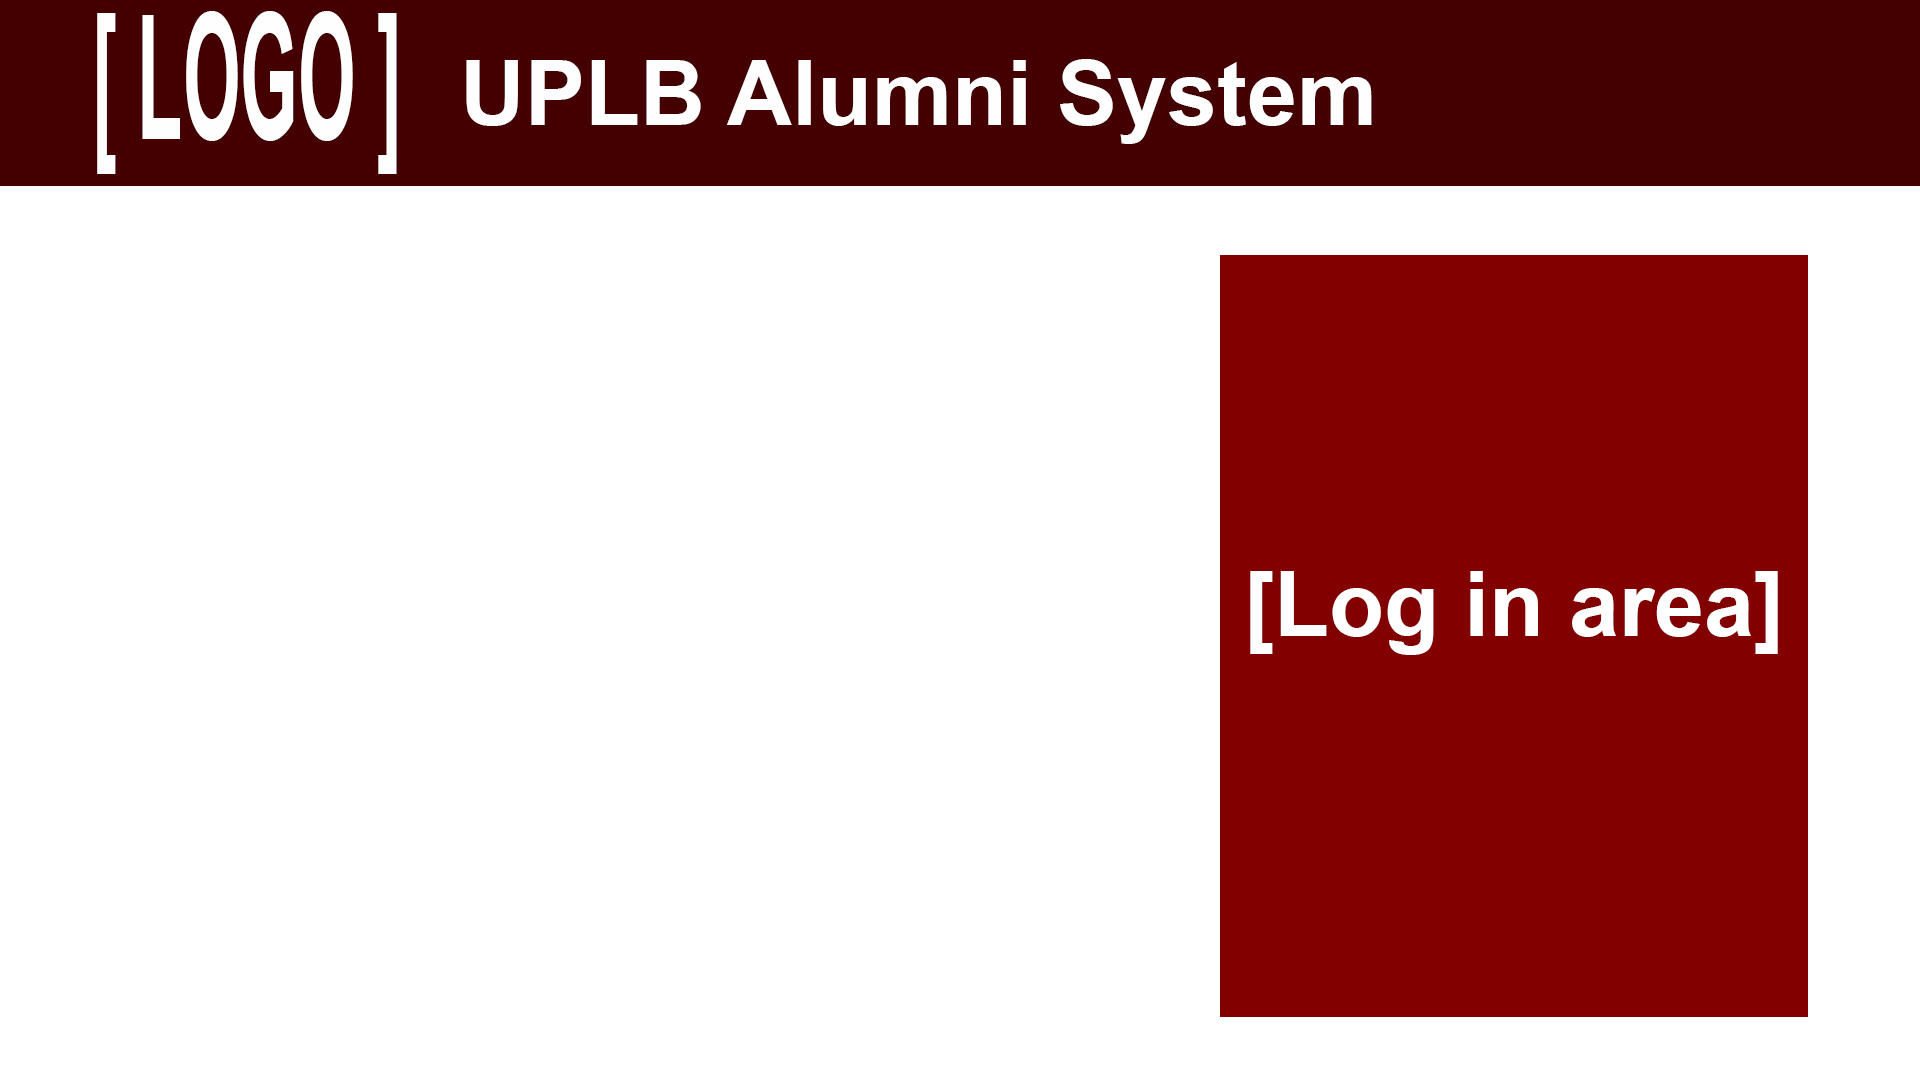
\includegraphics[height=50mm]{Images/MockupUI/Index.png}
		\caption{Login page}
\end{center}
\end{figure} 

\begin{figure}[H]
\begin{center}
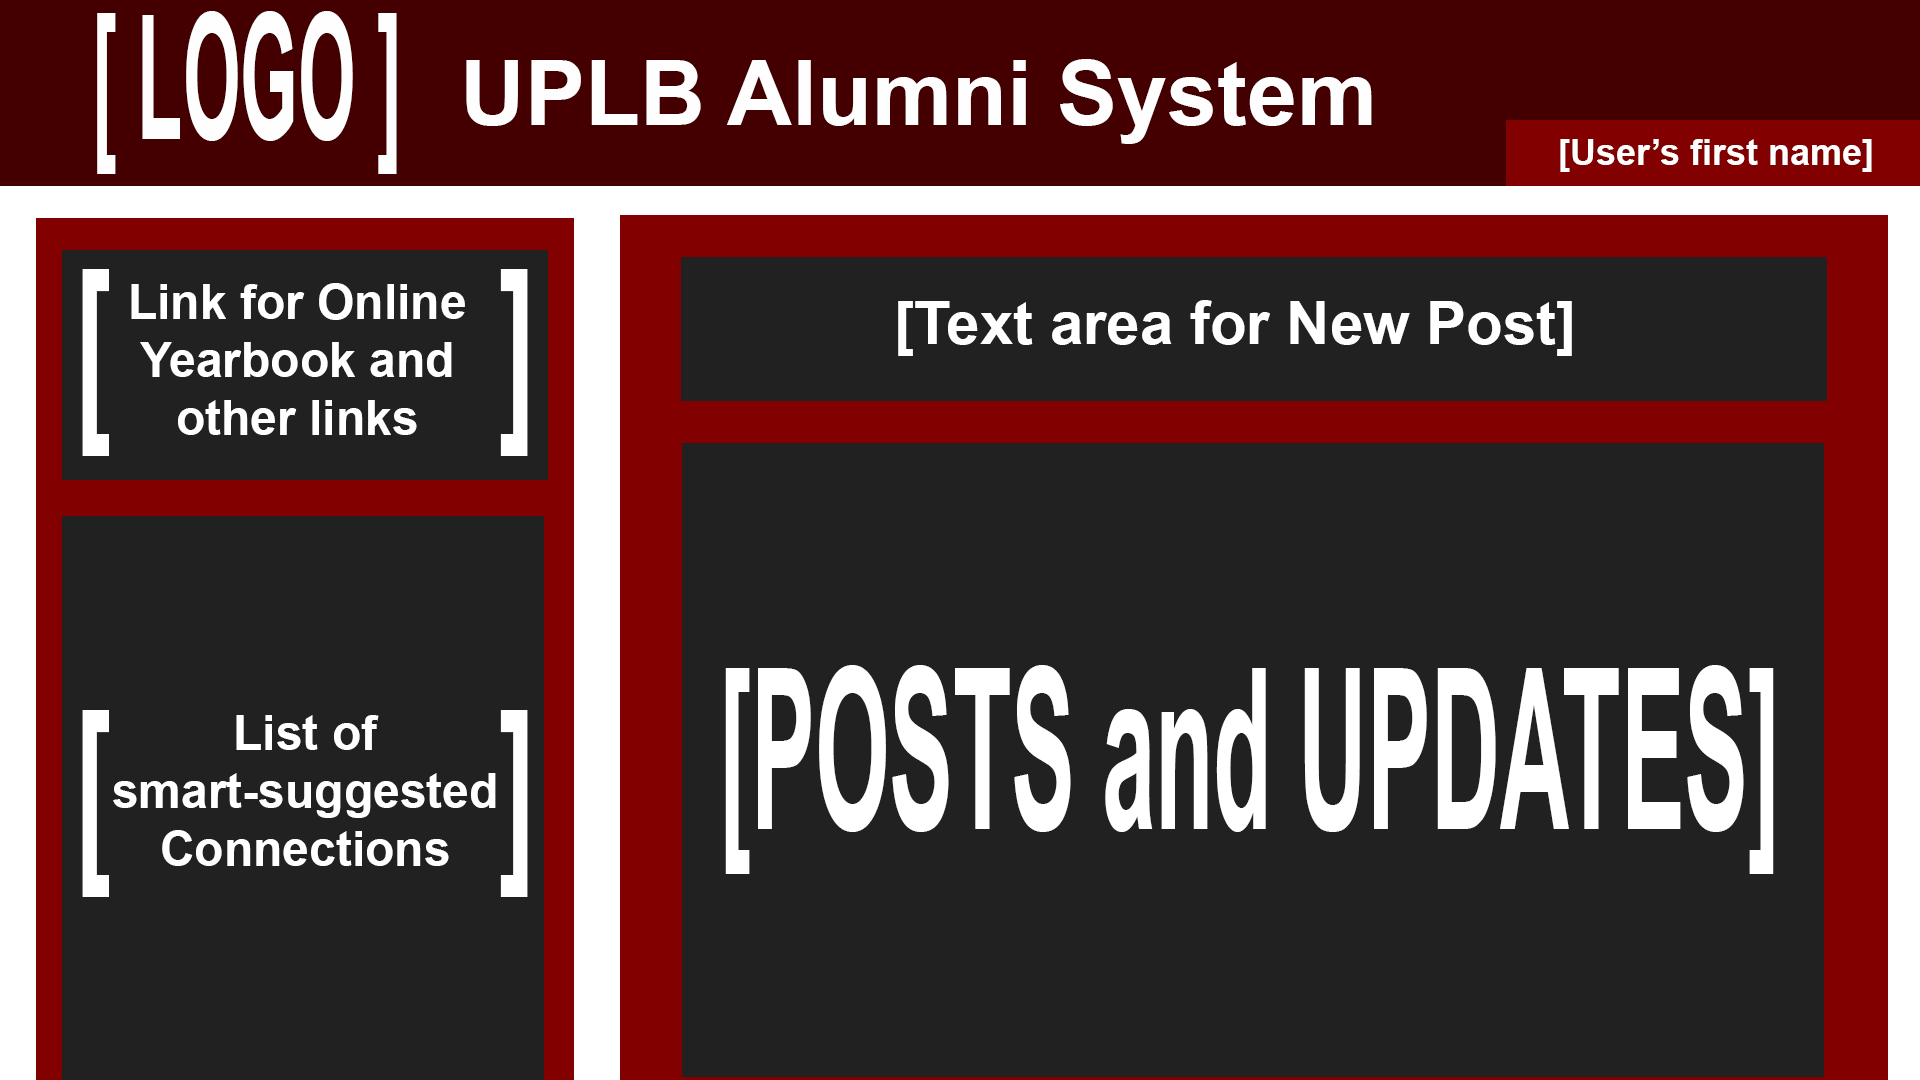
\includegraphics[height=50mm]{Images/MockupUI/UserHome.png}
\caption{Homepage for Alumni users}
\end{center}
\end{figure}

\begin{figure}[H]
\begin{center}
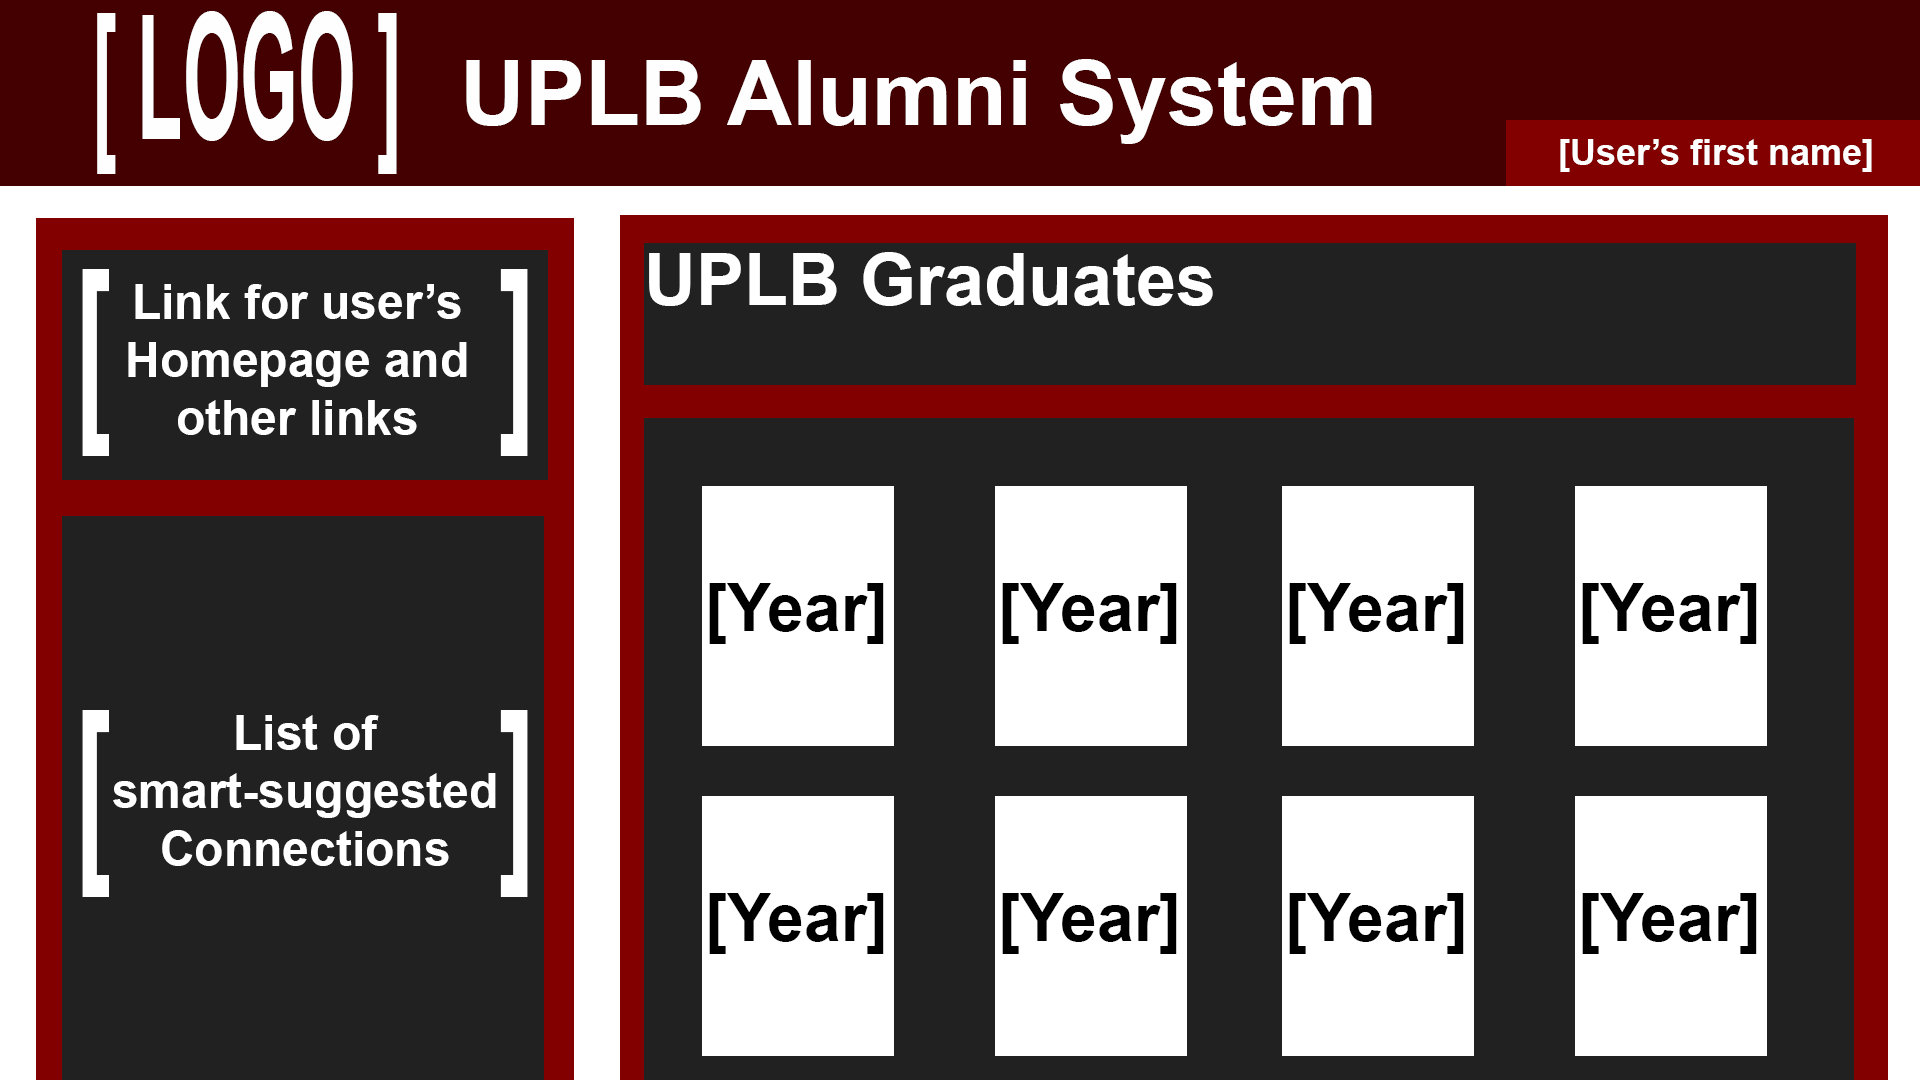
\includegraphics[height=50mm]{Images/MockupUI/OnlineYearbook.png}
\caption{Index page of the yearbook feature}
\end{center}
\end{figure}

\begin{figure}[H]
\begin{center}
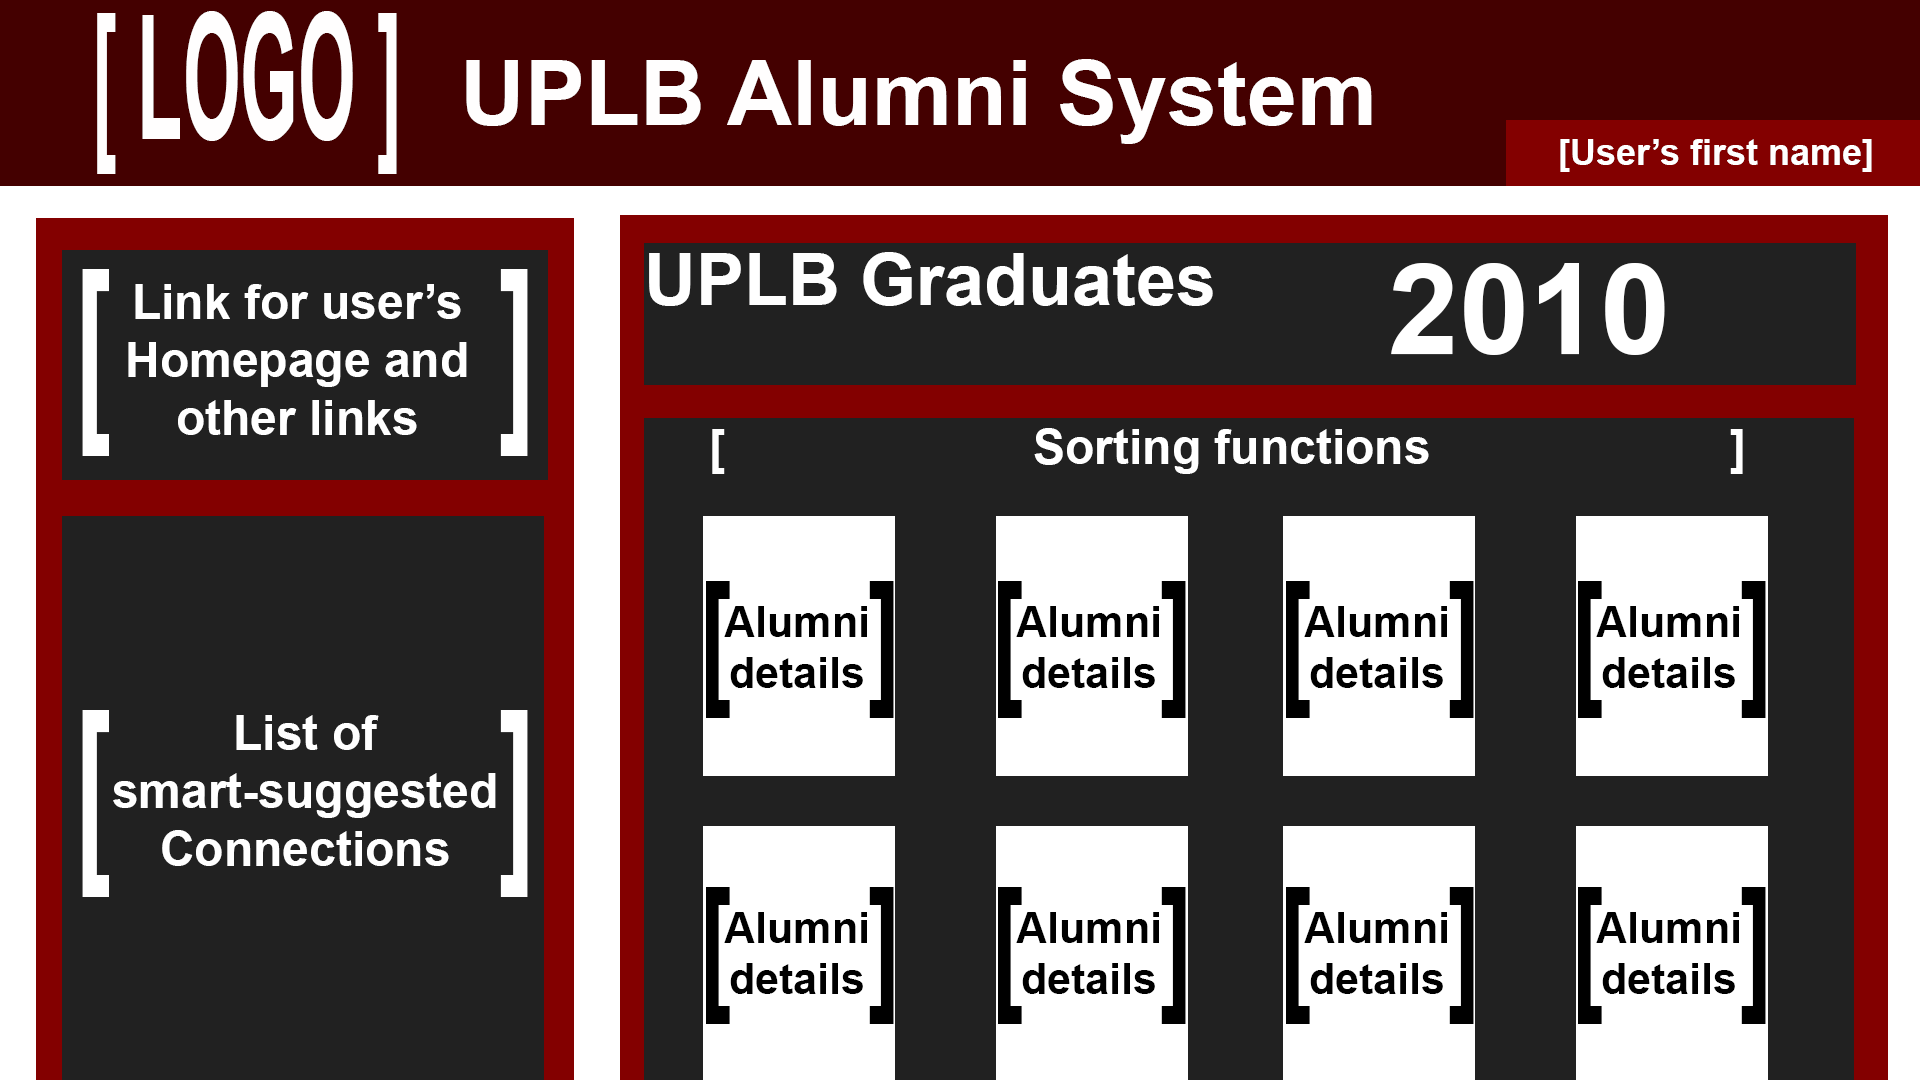
\includegraphics[height=50mm]{Images/MockupUI/OnlineYearbookYear.png}
\caption{View after selecting a year from the yearbook list}
\end{center}
\end{figure}


% BIBLIOGRAPHY
\bibliographystyle{./IEEE/IEEEtran}
\bibliography{./cs190-ieee}
% \nocite{*}

\end{document}